\documentclass[a4paper]{article}\usepackage{graphicx, color}
%% maxwidth is the original width if it is less than linewidth
%% otherwise use linewidth (to make sure the graphics do not exceed the margin)
\makeatletter
\def\maxwidth{ %
  \ifdim\Gin@nat@width>\linewidth
    \linewidth
  \else
    \Gin@nat@width
  \fi
}
\makeatother

\IfFileExists{upquote.sty}{\usepackage{upquote}}{}
\definecolor{fgcolor}{rgb}{0.2, 0.2, 0.2}
\newcommand{\hlnumber}[1]{\textcolor[rgb]{0,0,0}{#1}}%
\newcommand{\hlfunctioncall}[1]{\textcolor[rgb]{0.501960784313725,0,0.329411764705882}{\textbf{#1}}}%
\newcommand{\hlstring}[1]{\textcolor[rgb]{0.6,0.6,1}{#1}}%
\newcommand{\hlkeyword}[1]{\textcolor[rgb]{0,0,0}{\textbf{#1}}}%
\newcommand{\hlargument}[1]{\textcolor[rgb]{0.690196078431373,0.250980392156863,0.0196078431372549}{#1}}%
\newcommand{\hlcomment}[1]{\textcolor[rgb]{0.180392156862745,0.6,0.341176470588235}{#1}}%
\newcommand{\hlroxygencomment}[1]{\textcolor[rgb]{0.43921568627451,0.47843137254902,0.701960784313725}{#1}}%
\newcommand{\hlformalargs}[1]{\textcolor[rgb]{0.690196078431373,0.250980392156863,0.0196078431372549}{#1}}%
\newcommand{\hleqformalargs}[1]{\textcolor[rgb]{0.690196078431373,0.250980392156863,0.0196078431372549}{#1}}%
\newcommand{\hlassignement}[1]{\textcolor[rgb]{0,0,0}{\textbf{#1}}}%
\newcommand{\hlpackage}[1]{\textcolor[rgb]{0.588235294117647,0.709803921568627,0.145098039215686}{#1}}%
\newcommand{\hlslot}[1]{\textit{#1}}%
\newcommand{\hlsymbol}[1]{\textcolor[rgb]{0,0,0}{#1}}%
\newcommand{\hlprompt}[1]{\textcolor[rgb]{0.2,0.2,0.2}{#1}}%

\usepackage{framed}
\makeatletter
\newenvironment{kframe}{%
 \def\at@end@of@kframe{}%
 \ifinner\ifhmode%
  \def\at@end@of@kframe{\end{minipage}}%
  \begin{minipage}{\columnwidth}%
 \fi\fi%
 \def\FrameCommand##1{\hskip\@totalleftmargin \hskip-\fboxsep
 \colorbox{shadecolor}{##1}\hskip-\fboxsep
     % There is no \\@totalrightmargin, so:
     \hskip-\linewidth \hskip-\@totalleftmargin \hskip\columnwidth}%
 \MakeFramed {\advance\hsize-\width
   \@totalleftmargin\z@ \linewidth\hsize
   \@setminipage}}%
 {\par\unskip\endMakeFramed%
 \at@end@of@kframe}
\makeatother

\definecolor{shadecolor}{rgb}{.97, .97, .97}
\definecolor{messagecolor}{rgb}{0, 0, 0}
\definecolor{warningcolor}{rgb}{1, 0, 1}
\definecolor{errorcolor}{rgb}{1, 0, 0}
\newenvironment{knitrout}{}{} % an empty environment to be redefined in TeX

\usepackage{alltt}
\usepackage{a4wide}
\usepackage[margin=.8in]{geometry}
\usepackage{colortbl}

\title{Comparison of Versions of Kinship Links}
\author{Joe Rodger's BG Team}
\begin{document}
\maketitle

\definecolor{goodColor}{rgb}{.9,1,.85}
\definecolor{sosoColor}{rgb}{1,0.9215686,0.6117647}
\definecolor{badColor}{rgb}{1,.85,.85}
\definecolor{nullColor}{rgb}{.9, 0.85, 0.95} %0.8000000 0.7529412 0.8549020
\setlength{\parindent}{0pt}%http://tex.stackexchange.com/questions/49188/how-to-insert-vertical-space-between-paragraphs







% \textbf{RelationshipPaths Considered}: includedRelationshipPaths;\\
\textbf{Newer Links Version}: 53;
\textbf{Older Links Version}: 52;

\begin{knitrout}
\definecolor{shadecolor}{rgb}{0.969, 0.969, 0.969}\color{fgcolor}\begin{kframe}
\begin{verbatim}
Newer Links: ??? R Excludes Gen1 R=0, .375, .75
Older Links: After splitting off Gen1 Explicit tagset
\end{verbatim}
\end{kframe}
\end{knitrout}


\begin{figure}[htbp]
\begin{knitrout}
\definecolor{shadecolor}{rgb}{0.969, 0.969, 0.969}\color{fgcolor}
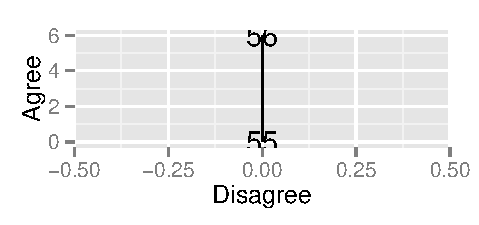
\includegraphics[width=\maxwidth]{figure/unnamed-chunk-31} 

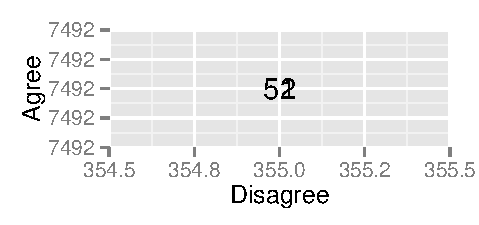
\includegraphics[width=\maxwidth]{figure/unnamed-chunk-32} 

\end{knitrout}

\caption{ROC for Gen1Housemates (left) and Gen2Siblings (right)}
\end{figure}

% latex table generated in R 2.15.3 by xtable 1.7-1 package
% Wed Mar 13 18:18:27 2013
\begin{table}[ht]
\centering
{\large
\begin{tabular}{lrrrrr}
  \hline
R & Implicit2004 & Implicit & Roster & Explicit & Eventual \\ 
  \hline
0 & - & - & 478 & - & - \\ 
  0.125 &  76 & - &  96 & - &  96 \\ 
  0.25 &  43 & - & - & 260 & 253 \\ 
  0.375 & 310 & - & - &  47 & - \\ 
  0.5 & 1877 & - & - & 3570 & 3548 \\ 
  0.75 &  32 & - & - & - & - \\ 
  1 & - & - & - & - &  11 \\ 
  - & 2964 & 5302 & 4728 & 1425 & 1394 \\ 
   \hline
\end{tabular}
}
\caption{Counts for Gen1Housemates} 
\end{table}
% latex table generated in R 2.15.3 by xtable 1.7-1 package
% Wed Mar 13 18:18:27 2013
\begin{table}[ht]
\centering
{\large
\begin{tabular}{lrrrrr}
  \hline
R & Implicit2004 & Implicit & Roster & Explicit & Eventual \\ 
  \hline
0 & - & - & 478 & - & - \\ 
  0.125 &  76 & - &  96 & - &  96 \\ 
  0.25 &  43 & - & - & 260 & 253 \\ 
  0.375 & 310 & - & - &  47 & - \\ 
  0.5 & 1877 & - & - & 3570 & 3548 \\ 
  0.75 &  32 & - & - & - & - \\ 
  1 & - & - & - & - &  11 \\ 
  - & 2964 & 5302 & 4728 & 1425 & 1394 \\ 
   \hline
\end{tabular}
}
\caption{Counts for Gen1Housemates (Previous version of links)} 
\end{table}
% latex table generated in R 2.15.3 by xtable 1.7-1 package
% Wed Mar 13 18:18:27 2013
\begin{table}[ht]
\centering
{\large
\begin{tabular}{lrrrr}
  \hline
R & Implicit2004 & Implicit & Explicit & Eventual \\ 
  \hline
0.25 & 2221 & 3012 & 2975 & 3442 \\ 
  0.375 & 2663 & - & 244 & 610 \\ 
  0.5 & 5778 & 6731 & 5599 & 6997 \\ 
  0.75 & - &  12 & - &  12 \\ 
  1 &  36 &  27 &  22 &  27 \\ 
  - & 390 & 1306 & 2248 &   0 \\ 
   \hline
\end{tabular}
}
\caption{Counts for Gen2Siblings} 
\end{table}
% latex table generated in R 2.15.3 by xtable 1.7-1 package
% Wed Mar 13 18:18:27 2013
\begin{table}[ht]
\centering
{\large
\begin{tabular}{lrrrr}
  \hline
R & Implicit2004 & Implicit & Explicit & Eventual \\ 
  \hline
0.25 & 2221 & 3012 & 2975 & 3442 \\ 
  0.375 & 2663 & - & 244 & 610 \\ 
  0.5 & 5778 & 6731 & 5599 & 6997 \\ 
  0.75 & - &  12 & - &  12 \\ 
  1 &  36 &  27 &  22 &  27 \\ 
  - & 390 & 1306 & 2248 &   0 \\ 
   \hline
\end{tabular}
}
\caption{Counts for Gen2Siblings (Previous version of links)} 
\end{table}


% 
% <<echo=FALSE, results='asis'>>=
% if( sum(ds$RelationshipPath==1) > 0 ) 
%   PrintConditionalTable(relationshipPathID=1, tabelCaption="Counts for Gen1Housemates")
% if( sum(ds$RelationshipPath==2) > 0 )
%   PrintConditionalTable(relationshipPathID=2, tabelCaption="Counts for Gen2Siblings")
% @

\end{document}
